\documentclass[12pt,a4paper]{article}

\usepackage[margin=1in]{geometry}\usepackage{graphicx}\usepackage{booktabs}\usepackage{float}\usepackage{setspace}\usepackage{hyperref}\onehalfspacing

\title{EfficientDet-D0 and EA-StrongSORT for Multi-Perspective Surgical Tool Tracking on CholecTrack20}

\author{Abdullah and Shamsa \textbackslash{} College of Engineering and Technology, American University in the Emirates}

\date{May 2026}

\begin{document}\maketitle

\begin{abstract}

This paper presents a deep learning framework for surgical tool detection and multi-perspective tracking on CholecTrack20. The problem is challenging because laparoscopic tools are small, reflective, frequently occluded, and can leave or re-enter the camera view. The study first evaluates YOLO11 as a detector baseline and then switches to EfficientDet-D0 after YOLO11 tuning shows limited improvement. EfficientDet-D0 uses an EfficientNet-B0 backbone with BiFPN weighted feature fusion and is integrated with EA-StrongSORT for tracking-by-detection. The selected detector achieved AP0.5 = 44.4, AP0.75 = 31.2, and AP0.5:0.95 = 27.9, improving over the internal YOLO11 baseline while trading away inference speed. Tracking evaluation on the eight CholecTrack20 test videos produced visibility, intracorporeal, and intraoperative MOTA values of 20.974, 19.641, and 19.314, respectively. The contribution is a reproducible EfficientNet-family detector-to-tracker baseline, a documented hyperparameter path, and an error analysis showing that detector quality and identity fragmentation remain the main limitations. These findings support future detector refinement before deeper tracker optimization.

\end{abstract}

\textbf{Keywords:} CholecTrack20; surgical tool tracking; EfficientDet; EfficientNet; EA-StrongSORT; transfer learning; multi-object tracking

\section{Introduction}

Computer-assisted surgery increasingly depends on the ability to interpret endoscopic video streams in real time. In laparoscopic cholecystectomy, the camera provides the primary view of the operative field, and the visible instruments encode important information about phase progression, surgeon actions, safety-critical interactions, and workflow interruptions. A system that can reliably detect and track surgical tools can therefore support downstream tasks such as surgical phase recognition, skill assessment, automatic video indexing, warning systems, and context-aware robotic assistance. Unlike ordinary object tracking, however, surgical tool tracking operates inside a constrained and visually unstable environment where instruments are metallic, reflective, thin, partially visible, and frequently occluded by tissue, smoke, blood, lens fouling, and other tools.

The CholecTrack20 paper argues that standard tracking formulations are not sufficient for this setting because surgical tools do not simply move continuously inside the camera view. A tool may disappear because the camera moves away from it, because the tool leaves the abdominal cavity, because it is hidden behind tissue, or because it remains physically present but outside the laparoscope's field of view. These cases have different clinical meanings, so CholecTrack20 defines three identity perspectives: visibility, intracorporeal, and intraoperative (Nwoye et al., 2025). Visibility tracking focuses on what is seen in the current camera field. Intracorporeal tracking preserves identity while the tool remains inside the patient. Intraoperative tracking preserves identity at the broader procedure level. This multi-perspective design makes the dataset more clinically expressive, but it also makes the tracking task significantly harder.

This project was built as an extension of that research direction. The central question was whether an EfficientNet-family detector integrated with a StrongSORT-style association pipeline could produce a useful baseline for CholecTrack20 surgical tool tracking. The project began with YOLO11 because YOLO-style detectors are strong real-time baselines and because the CholecTrack20 benchmark reports high performance for YOLOv7, YOLOv8, YOLOv9, and YOLOv10. After several YOLO11 tuning runs, the detector reached only modest accuracy on the validation split. The project therefore switched to EfficientDet-D0, which combines an EfficientNet-B0 backbone with a BiFPN feature-fusion detector head (Tan et al., 2020).

The second motivation came from the EA-StrongSORT paper provided as reference. That paper follows a detection-based tracking paradigm and improves StrongSORT by replacing the conventional ReID feature extractor with a lightweight EfficientNetV2-based backbone, adding Efficient Channel Attention, and improving spatial association through GIoU-style matching (Ghatwary et al., n.d.). Although that work targets tumor tracking in cine-MRI rather than surgical tools in laparoscopic video, the conceptual overlap is strong: both problems require frame-level detection followed by temporally stable identity association under appearance change, motion, and real-time constraints.

The research gap addressed in this report is the lack of a documented EfficientNet-family detector-to-tracker study on CholecTrack20. The public CholecTrack20 benchmark is dominated by YOLO-style detector results and modern tracking baselines, while the EA-StrongSORT reference motivates EfficientNet-based appearance learning in a different medical tracking domain. This creates a useful middle ground for investigation: EfficientNet can be tested in the detection stage through EfficientDet-D0, and StrongSORT-style association can be evaluated on the three CholecTrack20 identity perspectives. The result is a project that is not simply a reproduction of the public benchmark but a controlled contribution exploring whether EfficientNet-based design choices transfer usefully to surgical tool tracking.

The contribution of this paper is therefore not a claim of state-of-the-art performance. Instead, it is a reproducible experimental study showing the path from YOLO11 baseline experiments to an EfficientDet-D0 detector feeding a StrongSORT/EA-StrongSORT-oriented tracking pipeline on CholecTrack20. The work documents detector hyperparameter decisions, compares YOLO11 and EfficientDet-D0 using CholecTrack20-style metrics, runs full test-set tracking, and analyzes why the resulting tracker remains far behind the strongest public baselines. This is important because a negative or moderate result can still be scientifically useful when it identifies the bottleneck and creates a transparent baseline for the next design iteration.

\section{Related Work}

Surgical video understanding has developed rapidly because laparoscopic and endoscopic videos contain rich procedural information. Early surgical tool studies often focused on frame-level recognition or detection, where the objective was to identify whether a tool was present and localize it with a bounding box. This is useful, but it does not fully describe temporal behavior. Surgical actions are inherently sequential: a tool enters, interacts with tissue, changes role, disappears, and may return later. Tracking is therefore a natural extension because it connects detections through time and assigns identities that can be used to reason about tool usage, hand assignment, and procedural state.

CholecTrack20 addresses a gap in earlier surgical tool datasets by providing full-length videos and multi-perspective tracking annotations (Nwoye et al., 2025). The dataset includes seven tool categories and records additional surgical context such as operator, phase, visual challenge, and three different identity perspectives. The CholecTrack20 authors emphasize that many existing datasets treat surgical tracking too generically, whereas clinical interpretation depends on whether a tool is only temporarily outside the field of view, fully outside the body, or still part of the same operative action. This makes CholecTrack20 more demanding than a conventional multi-object tracking dataset and gives it a closer connection to real surgical workflow analysis.

Object detection has traditionally been divided into two-stage and one-stage families. Two-stage approaches such as Faster R-CNN generate candidate regions and then classify or refine them, often achieving strong localization accuracy at the cost of speed. One-stage approaches such as YOLO directly predict boxes and classes in a single pass, which makes them attractive for real-time systems (Redmon et al., 2016). Modern YOLO variants have improved the balance between speed and accuracy through better backbones, necks, training strategies, and label assignment. The CholecTrack20 benchmark shows that YOLOv7 through YOLOv10 are especially strong on this dataset, with AP0.5:0.95 values above 55 for the best reported configurations.

The initial use of YOLO11 in this project was motivated by that trend. YOLO-style detectors are practical because they are fast, widely supported, and easy to integrate with tracking-by-detection frameworks. However, detector performance is highly sensitive to training data size, class imbalance, image resolution, optimizer settings, and domain shift. In this project, YOLO11 showed excellent speed but limited AP on CholecTrack20 validation data. That result motivated the shift toward an EfficientNet-family detector rather than more YOLO-only tuning.

EfficientNet introduced compound scaling, where network depth, width, and input resolution are scaled together rather than independently (Tan \& Le, 2019). This design principle is useful when hardware resources are limited, because it seeks a better accuracy-efficiency trade-off than simply making a network deeper or wider. EfficientDet extends EfficientNet to object detection by combining an EfficientNet backbone with a bidirectional feature pyramid network, or BiFPN (Tan et al., 2020). BiFPN performs weighted multi-scale feature fusion, allowing the detector to learn how much information to use from different feature resolutions. This is valuable for laparoscopic tools because some detections correspond to large visible shafts while others correspond to small tips or partially visible fragments.

Attention mechanisms are also relevant to this project. In EfficientDet, BiFPN's learned feature fusion acts as a scale-level attention mechanism because it assigns relative importance to different feature-map paths. In the EA-StrongSORT paper, attention appears in the tracking stage through Efficient Channel Attention inserted into deeper EfficientNetV2 blocks (Ghatwary et al., n.d.; Wang et al., 2020). ECA is designed to improve channel-wise feature selection without large computational overhead. For ReID embeddings, this matters because identity association depends on subtle appearance cues that may be hidden by noise, deformation, or partial visibility.

The difference between surgical tool tracking and tumor tracking also deserves attention. In cine-MRI tumor tracking, the object of interest is usually a single anatomical region with low contrast and non-rigid motion. In surgical tool tracking, the objects are multiple rigid metallic instruments with sharp geometry, specular highlights, repeated class appearances, and frequent crossings. The imaging modalities are different, but both settings penalize unstable temporal association. This is why the EA-StrongSORT paper is a useful methodological reference even though its dataset is TrackRAD2025 rather than CholecTrack20. It justifies focusing on lightweight detection, discriminative appearance embeddings, and robust association metrics rather than treating each frame independently.

Tracking-by-detection is the dominant practical formulation for many multi-object tracking systems. The detector first produces candidate object boxes for each frame, and the tracker associates those boxes over time. SORT is a simple and influential method that combines a Kalman filter for motion prediction with Hungarian matching for assignment (Bewley et al., 2016). DeepSORT extends SORT by adding appearance embeddings, making it more robust when objects cross, disappear briefly, or have similar motion (Wojke et al., 2017). StrongSORT further improves association and appearance modeling, making it a strong baseline for tracking-by-detection systems (Du et al., 2023).

Recent trackers also show that association strategy matters as much as detection. ByteTrack associates high-confidence and low-confidence detections in separate stages, reducing missed objects when detector confidence drops (Zhang et al., 2022). Bot-SORT combines motion and appearance cues with camera-motion compensation, leading to strong results in many benchmark settings (Aharon et al., 2022). CholecTrack20 reports that Bot-SORT and ByteTrack are strong public baselines, especially in visibility tracking. However, the benchmark also shows that performance drops under stricter perspectives and difficult surgical visual challenges, so identity preservation remains unresolved.

EA-StrongSORT is particularly relevant because it explicitly modifies StrongSORT rather than replacing the tracking-by-detection paradigm. The reference EA-StrongSORT paper argues that the original ReID backbone can be computationally heavy and that stronger lightweight embeddings can improve temporal association. Its proposed changes include an EfficientNetV2-based feature extractor, selective ECA attention in deeper layers, and GIoU-based spatial association. The paper's ablation study reports that each component improves MOTA and HOTA compared with original StrongSORT. This provides the design rationale for using StrongSORT-style association in the present project and for proposing a future exact EA-StrongSORT ReID replacement after the detector bottleneck is improved.

\section{Proposed Methodology}

The proposed framework follows a tracking-by-detection architecture. Each input video is decoded frame by frame. The detector receives the preprocessed frame and predicts bounding boxes, confidence values, and surgical tool classes. These detections are converted into the tracker format [x1, y1, x2, y2, confidence, class]. The tracking module then associates detections across consecutive frames and writes MOT-format prediction files. Finally, the predictions are evaluated against CholecTrack20 ground truth under visibility, intracorporeal, and intraoperative perspectives. This modular architecture was selected because it allows the detector and tracker to be studied separately while still producing an end-to-end pipeline.

The detector used in the final pipeline is EfficientDet-D0. It was selected because it is the smallest EfficientDet family member and is therefore feasible on the available RTX 2060 GPU with 6 GB VRAM. EfficientDet-D0 uses an EfficientNet-B0 backbone pretrained on COCO and a BiFPN neck for multi-scale feature fusion. The detection head was replaced for seven CholecTrack20 tool classes. Transfer learning was performed by fine-tuning the detector on the converted CholecTrack20 YOLO-format training labels. Full fine-tuning was used instead of freezing the backbone because surgical endoscopic imagery differs substantially from COCO images in color distribution, geometry, illumination, object texture, and class appearance.

The detector training path was deliberately empirical. YOLO11 was first trained and evaluated because the CholecTrack20 benchmark strongly favors modern YOLO variants. Several YOLO11 configurations were tested, including SGD versus AdamW, 640 versus 768 image size, and different patience settings. Once the best YOLO11 run plateaued near AP0.5:0.95 = 26.6, EfficientDet-D0 was introduced. EfficientDet hyperparameter screening then varied learning rate, optimizer, image size, batch size, gradient accumulation, and validation interval. The final EfficientDet configuration used image size 640, AdamW, lr0 = 0.0002, lrf = 0.01, batch = 6, accumulation = 2, and 150 training epochs.

The attention mechanism in the detector is the BiFPN weighted feature fusion. Instead of simply adding feature maps from different pyramid levels, BiFPN learns normalized weights for each input feature path. This allows the model to emphasize the feature scale that is most useful for a specific detection. In surgical videos, this is important because tool appearance changes dramatically with distance and occlusion. A grasper shaft may occupy a large diagonal region, while a small visible tip may represent the only detectable evidence of the tool. Weighted multi-scale fusion gives the detector a mechanism for balancing these cases.

The tracking stage follows the StrongSORT family. StrongSORT maintains active tracks using motion prediction and appearance-based association. Motion prediction estimates where an existing track is expected to appear in the next frame, while appearance embeddings help distinguish tools when multiple instruments overlap or move similarly. The implementation used the BoxMOT StrongSORT tracker with OSNet ReID embeddings. In the project documentation this is treated as an EA-StrongSORT-oriented baseline because the experimental direction is based on the EA-StrongSORT paper, but the exact EfficientNetV2/ECA ReID replacement remains a future extension. This distinction is important: the present contribution replaces and studies the detector while preserving a stable StrongSORT association stage.

The EA-StrongSORT reference paper influenced the tracker design rationale in three ways. First, it supports the decision to keep a detection-based formulation rather than switching to segmentation, because detection-based tracking is lighter and easier to run frame-by-frame. Second, it shows why ReID backbone design matters: identity association is not only a box-overlap problem but also an appearance representation problem. Third, its use of GIoU-style spatial matching suggests a possible improvement over standard IoU association when boxes are close but not perfectly overlapping. These insights guide the discussion and future-work plan for adapting EA-StrongSORT more completely to surgical videos.

To avoid the memory issues encountered with long test videos, the project added a streaming EfficientDet-to-StrongSORT adapter. Rather than asking BoxMOT to load the detector through its command-line detector registry, frames are read directly, EfficientDet inference is run frame-by-frame, detections are passed into StrongSORT, and MOT rows are written incrementally. This design prevents long result lists from accumulating in memory and makes full CholecTrack20 benchmarking possible on the available workstation. It also supports smoke testing through video selection and frame stride, which was essential for debugging before running the full 12-hour benchmark.

\begin{figure}[H]\centering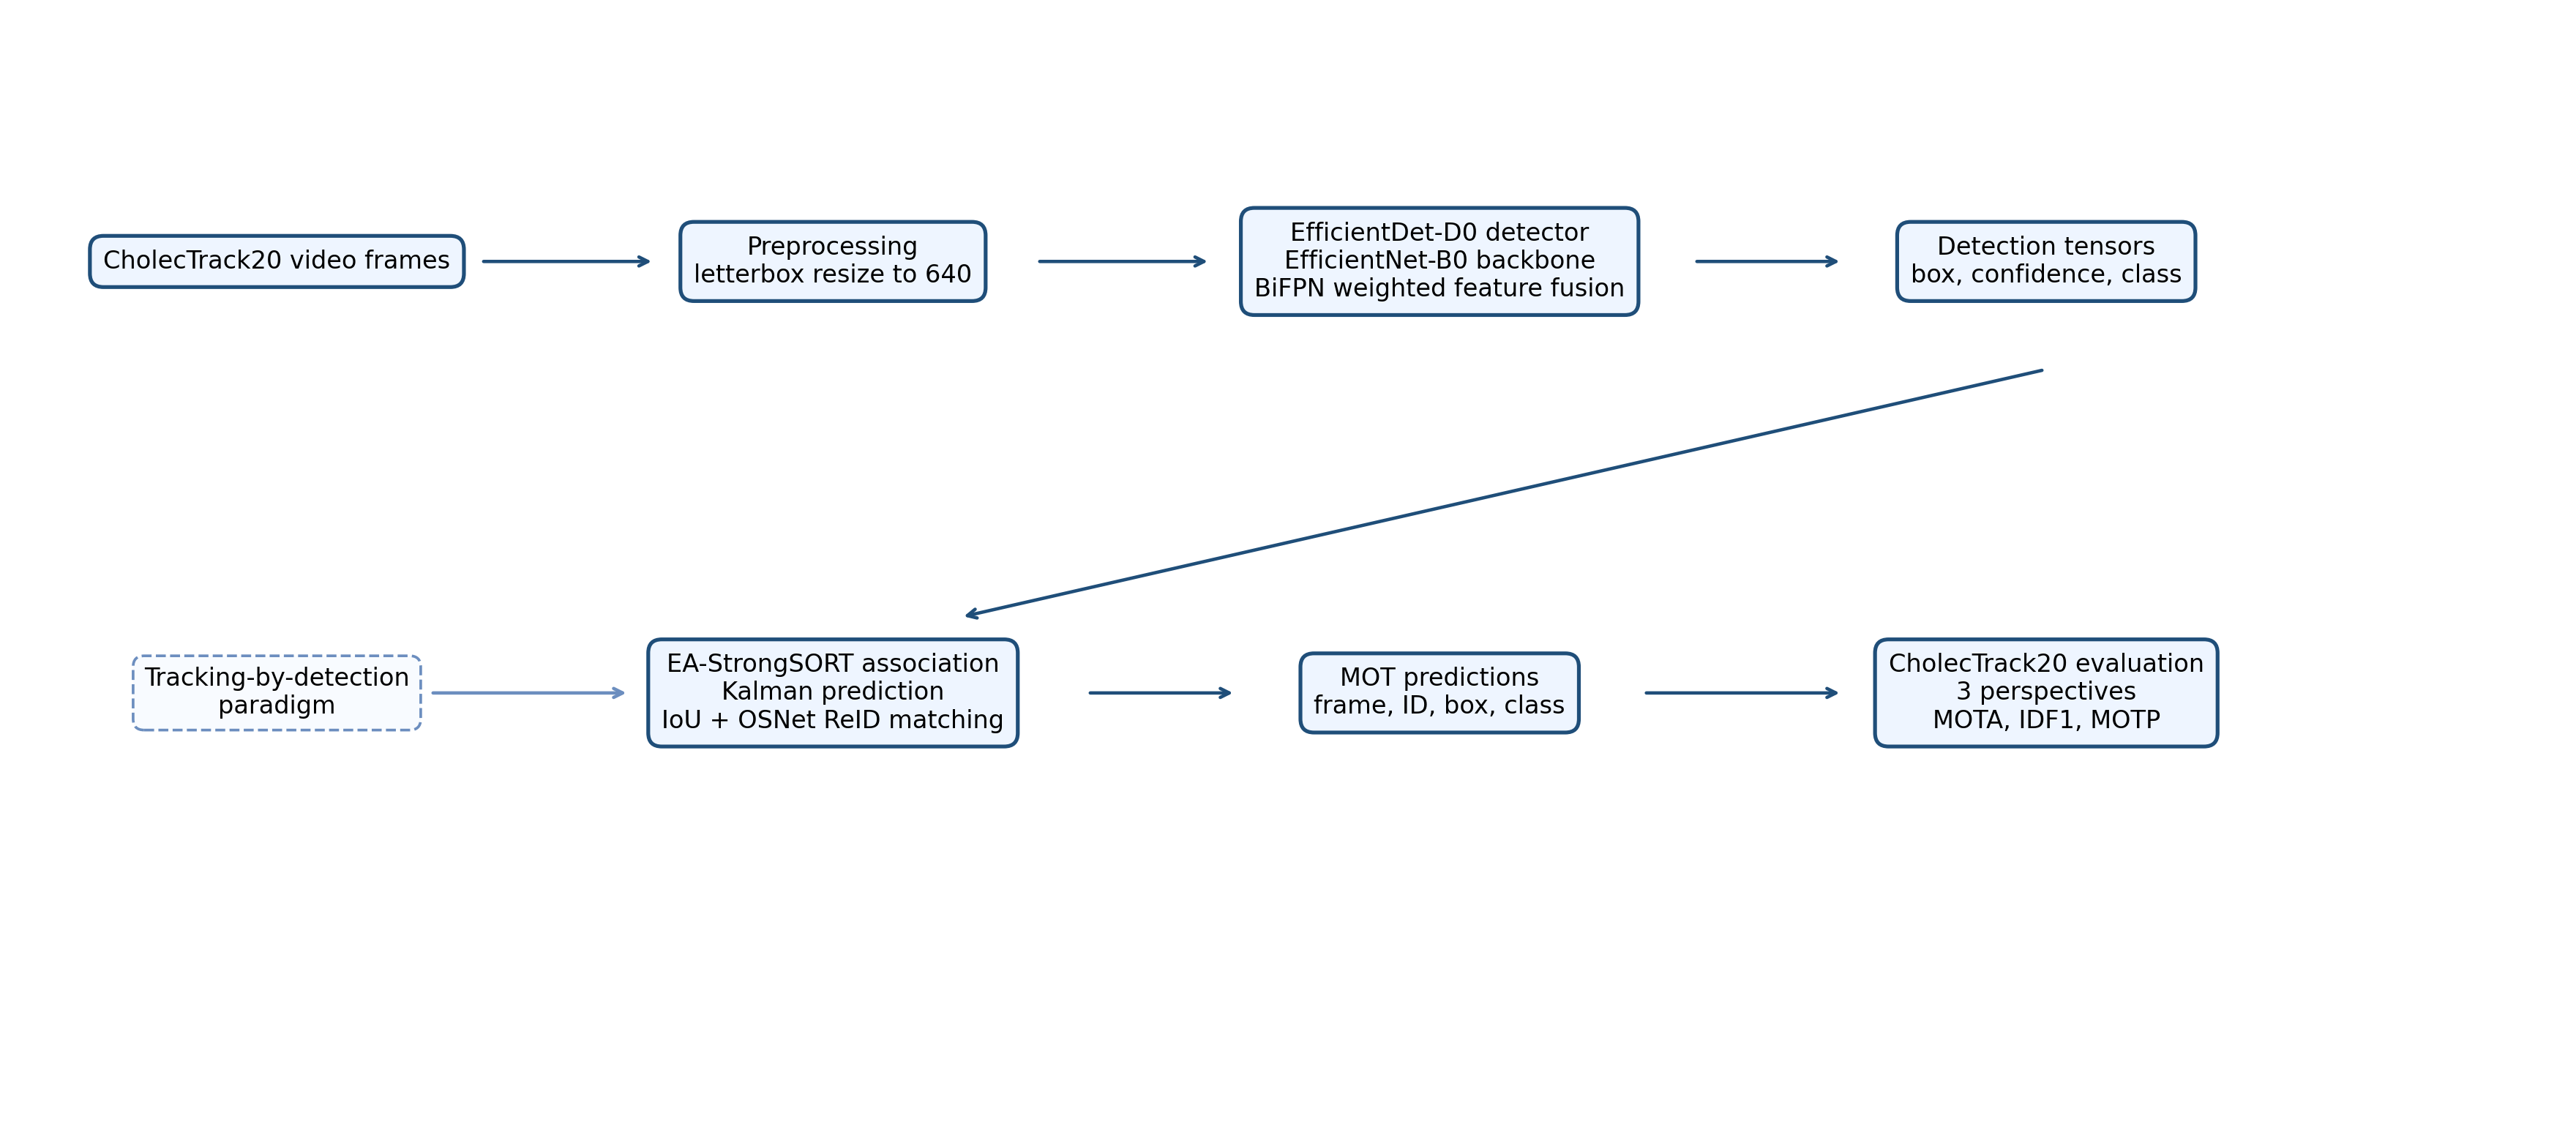
\includegraphics[width=\textwidth]{assets/architecture_diagram.png}\caption{Proposed EfficientDet-D0 to EA-StrongSORT architecture.}\end{figure}

\section{Dataset Description}

CholecTrack20 consists of 20 full-length laparoscopic cholecystectomy videos with surgical tool annotations. The dataset is designed for detection and tracking rather than only frame-level classification. It contains seven surgical tool categories: grasper, bipolar, hook, scissors, clipper, irrigator, and specimen bag. The original annotations include bounding boxes, class labels, track identities, operator information, surgical phase, and visual challenge labels. This makes the dataset unusually rich for a student project because it enables detector evaluation, tracking evaluation, category-level analysis, and analysis under difficult surgical conditions.

The project used the official procedure-level split: 10 training videos, 2 validation videos, and 8 testing videos. Keeping the split at the procedure level is important because frames from the same surgery are visually correlated. If frames from one operation appeared in both training and validation, the detector could overestimate its generalization ability. The final tracking evaluation used the Testing split, which contains VID01, VID06, VID07, VID111, VID12, VID25, VID39, and VID92. These videos were processed end-to-end to produce tracking predictions for all annotated frames.

The validation split used for detector selection contains 2,461 labelled frames and 4,106 tool instances. Its class distribution is imbalanced: grasper = 1,887, bipolar = 157, hook = 1,467, scissors = 56, clipper = 116, irrigator = 115, and specimen bag = 308. The imbalance is severe: grasper and hook dominate the validation distribution, while scissors, clipper, irrigator, and bipolar have far fewer instances. This is not just a statistical detail; it directly affects model behavior. The detector sees many more examples of common tools and has fewer opportunities to learn rare tools under smoke, blur, occlusion, and reflection.

CholecTrack20 also introduces perspective-specific identities. The visibility perspective is the closest to conventional video tracking because an identity is tied to a visible tool instance in the field of view. The intracorporeal perspective is stricter because identity may persist even when a tool temporarily leaves the camera view but remains inside the abdominal cavity. The intraoperative perspective is the broadest, preserving identity across the procedure-level role of the tool. These definitions mean that the same detection predictions can produce different tracking scores depending on how ground-truth identity continuity is interpreted.

For detector training, the original annotations were converted into YOLO-style label files. This format was useful because it allowed the same dataset conversion to support both the initial YOLO11 experiments and the later EfficientDet implementation. For tracking evaluation, however, the original CholecTrack20 identity annotations were preserved because the tracker must be assessed against visibility\_track, intracorporeal\_track, and intraoperative\_track fields. This separation between detector labels and tracker labels prevented accidental loss of identity information during preprocessing.

Preprocessing used letterbox resizing to maintain aspect ratio and fit frames into the selected model resolution. The final EfficientDet run used image size 640. Letterbox resizing was chosen because surgical tools are thin and elongated; arbitrary stretching could distort tool geometry and make bounding boxes less meaningful. Heavy random augmentation was not enabled in the selected final run. This was a conservative choice: because the project objective was to compare detector families and build a stable tracking pipeline, the final reported results use geometry-preserving preprocessing. Future work should test controlled photometric augmentation for smoke, blur, blood, and reflection robustness.

\section{Experimental Setup}

Experiments were run on a Windows workstation with an NVIDIA GeForce RTX 2060 GPU with 6 GB VRAM. The software stack used a Conda environment with PyTorch, torchvision, effdet, timm, OpenCV, BoxMOT, SciPy, and COCO-style evaluation tools. The hardware constraint was important throughout the project. EfficientDet-D0 was selected partly because larger EfficientDet variants and overly large batch sizes risked out-of-memory failures or very slow training. The final setup therefore balances experimental seriousness with the limits of a student workstation.

Training speed was treated as an engineering problem rather than an afterthought. Early YOLO11 and tracking experiments showed that full runs could take many hours, so the codebase was extended with quick, tune, smoke, and final presets. Smoke presets processed fewer videos or fewer frames to confirm that the pipeline worked. Tune presets used faster validation intervals and stable output names for hyperparameter comparison. Final runs used full validation and complete output artifacts. This workflow made it possible to debug efficiently while preserving a clean path to reportable results.

The selected EfficientDet-D0 training configuration used AdamW, lr0 = 0.0002, lrf = 0.01, weight decay = 0.0001, image size = 640, batch = 6, accumulation = 2, workers = 6, epochs = 150, patience = 30, AMP enabled, and validation every 3 epochs during tuning. Gradient accumulation produced an effective batch size of 12 without exceeding GPU memory. The learning rate schedule used a 3-epoch warmup followed by cosine annealing to the final learning-rate factor. This configuration was selected after screening lower learning rate, SGD, and 512-resolution alternatives.

Detector evaluation followed CholecTrack20-style metrics. The main columns are AP0.5, AP0.75, and AP0.5:0.95. AP0.5 measures detection quality under a looser IoU threshold, AP0.75 requires tighter localization, and AP0.5:0.95 averages over multiple IoU thresholds to provide a stricter summary. The paper-style detector evaluation also reports AP0.5 by tool category, AP across visual challenges, and FPS. This matters because a detector can have a reasonable global AP while still failing on a rare class or under a clinically relevant visual condition.

Tracking metrics include MOTA, IDF1, MOTP, precision, recall, false positives, false negatives, and identity switches. MOTA is sensitive to false positives, false negatives, and identity switches. IDF1 focuses more directly on identity preservation. MOTP measures localization precision among matched detections. In this project, tracking evaluation used class-aware IoU >= 0.5 matching on annotated CholecTrack20 frames. Class-agnostic evaluation was also computed as a diagnostic to determine whether poor performance came mainly from class-label errors or from missed detections and identity fragmentation.

The full tracking benchmark was computationally expensive. The final EfficientDet-D0 to StrongSORT run processed all eight test videos and produced MOT prediction files under the project logs. The run took approximately 12 hours, which is consistent with the detector speed, video length, and StrongSORT association overhead. This long runtime is one reason the project includes smoke commands and stride-based tests: final tracking should be run only after the detector appears worth evaluating.

\begin{table}[H]\centering\small\resizebox{\textwidth}{!}{%
\begin{tabular}{lllllll}
\toprule
Run & Settings & Best epoch & Precision & Recall & mAP50 & mAP50-95 \\ \midrule
final\_yolo11\_img768\_sgd & SGD, imgsz=768, batch=8, lr0=0.01 & 42 & 0.5595 & 0.4683 & 0.4077 & 0.2670 \\
final\_yolo11\_patience30 & SGD, imgsz=640, batch=16, lr0=0.01 & 31 & 0.5700 & 0.4715 & 0.4108 & 0.2631 \\
final\_yolo11\_adamw\_lr001 & AdamW, imgsz=640, batch=16, lr0=0.001 & 44 & 0.5573 & 0.4716 & 0.4035 & 0.2519 \\
\bottomrule
\end{tabular}}
\caption{YOLO11 baseline experiments.}
\end{table}

\begin{table}[H]\centering\small\resizebox{\textwidth}{!}{%
\begin{tabular}{llllllll}
\toprule
Selected & Run & Epochs & Best epoch & AP0.5 & AP0.75 & AP0.5:0.95 & FPS \\ \midrule
yes & efficientdet\_d0\_640\_adamw\_lr2e4\_long & 150 & 63 & 44.4 & 31.3 & 27.9 & 20.9 \\
no & efficientdet\_d0\_512\_adamw\_lr2e4\_batch12\_workers6\_eval3 & 100 & 96 & 46.6 & 28.5 & 27.2 & 28.8 \\
no & screen\_effdet\_d0\_640\_lr2e4 & 30 & 30 & 42.9 & 29.3 & 26.6 &  \\
no & screen\_effdet\_d0\_640\_lr1e4 & 30 & 30 & 41.2 & 28.9 & 25.7 &  \\
no & screen\_effdet\_d0\_sgd\_lr1e3 & 30 & 20 & 37.3 & 22.9 & 21.8 &  \\
\bottomrule
\end{tabular}}
\caption{EfficientDet-D0 hyperparameter screening.}
\end{table}

\begin{figure}[H]\centering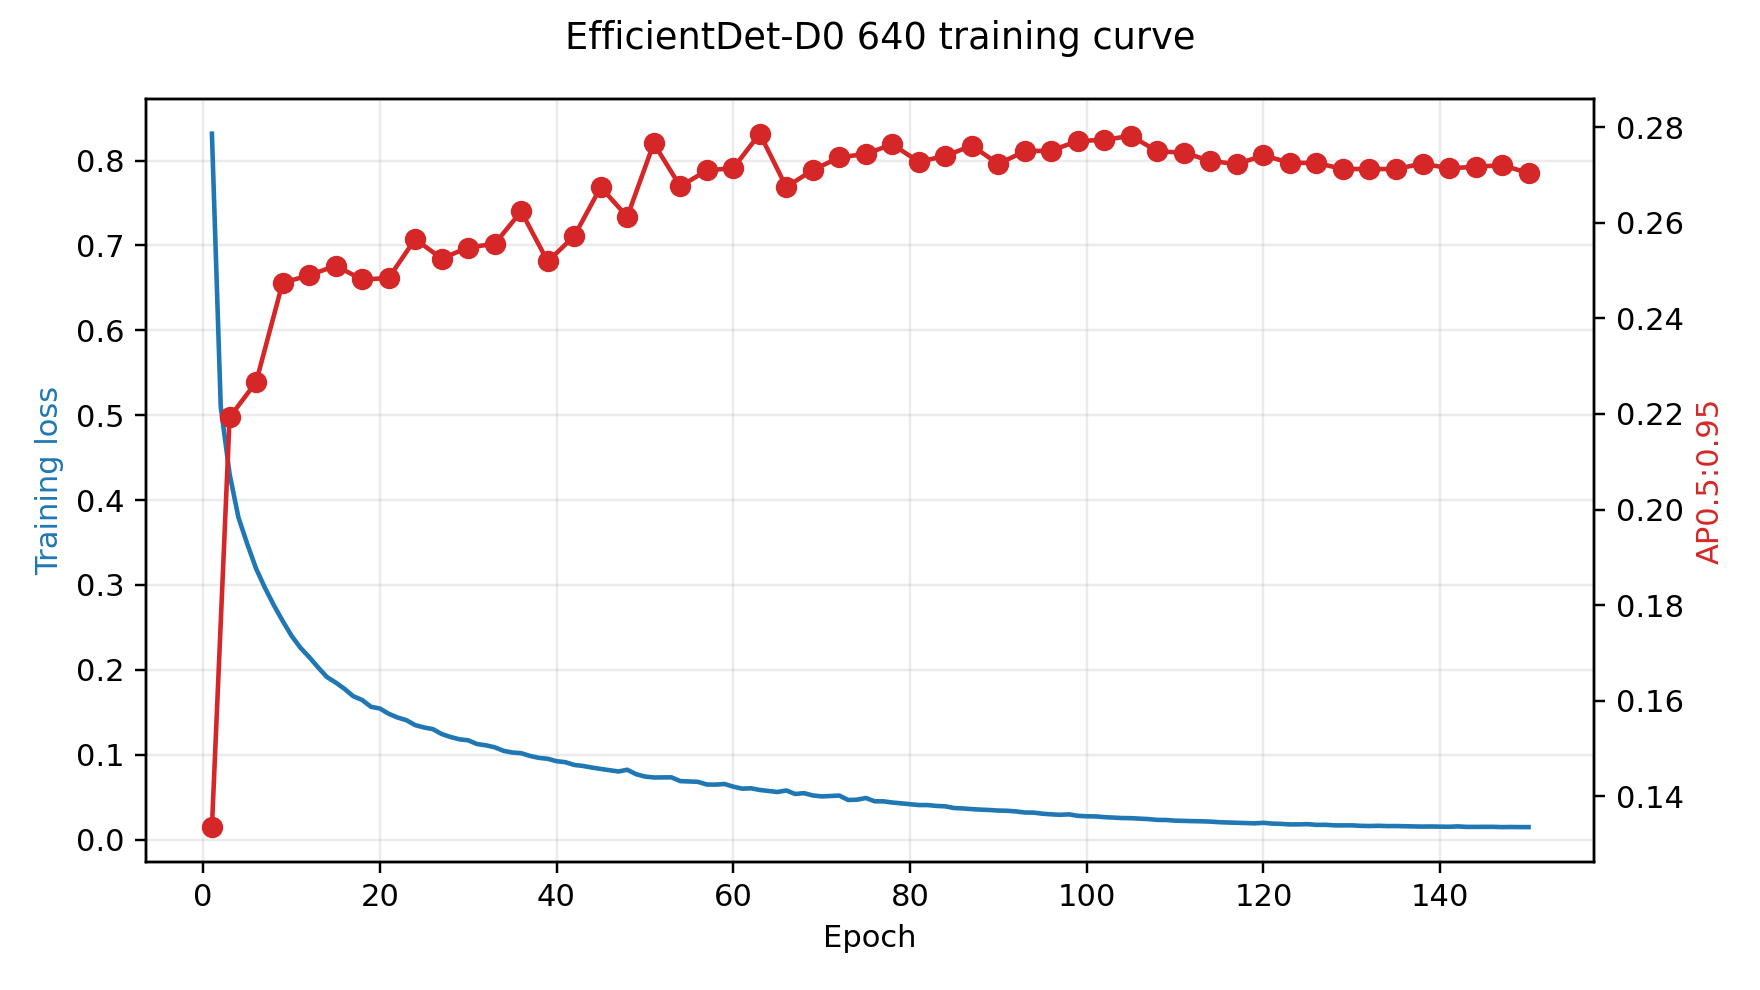
\includegraphics[width=0.9\textwidth]{assets/training_curve.png}\caption{EfficientDet-D0 training loss and AP curve.}\end{figure}

\section{Results and Discussion}

The YOLO11 baseline established an important starting point. Among the tested YOLO11 runs, SGD with image size 768 produced the best internal detector result. Increasing image size from 640 to 768 improved mAP50-95 only slightly, from 0.2631 to 0.2670, while AdamW underperformed the SGD configuration. The best YOLO11 paper-style AP0.5:0.95 was 26.6. This result was disappointing compared with the official CholecTrack20 YOLOv7-v10 benchmark, but it was useful because it showed that simply training the available YOLO11 configuration was not enough.

EfficientDet-D0 improved the internal baseline to AP0.5 = 44.4, AP0.75 = 31.2, and AP0.5:0.95 = 27.9. The improvement over YOLO11 was moderate: +4.1 AP0.5, +1.6 AP0.75, and +1.3 AP0.5:0.95. This means EfficientDet-D0 was selected because it was the best detector obtained in this project and because it satisfied the EfficientNet-family contribution goal. It should not be interpreted as closing the gap to the strongest public leaderboard models. The public YOLOv7-v10 results remain far higher, which suggests that the main bottleneck is still detector training quality and possibly dataset handling rather than tracker design alone.

The direct comparison between YOLO11 and EfficientDet-D0 reveals a clear trade-off. YOLO11 was much faster at 62.9 FPS, while EfficientDet-D0 reached 20.9 FPS. In applications where latency is the only priority, YOLO11 would be preferable. However, EfficientDet-D0 improved several clinically relevant subsets, including hook, scissors, bleeding, smoke, occlusion, foul lens, and trocar-related challenge categories. The largest class improvement was hook AP0.5, which increased from 50.0 to 60.3. Scissors also improved from 23.6 to 33.4. These improvements support the decision to continue the project with EfficientDet-D0 despite the lower FPS.

The most persistent detector weakness was the irrigator class. YOLO11 achieved only 3.4 AP0.5 for irrigator, and EfficientDet-D0 dropped to 0.6. This is not likely to be solved by a small optimizer adjustment. The validation distribution contains only 115 irrigator instances, and the tool can be visually ambiguous or partially visible. A stronger future detector study should therefore consider class-aware sampling, targeted augmentation, loss reweighting, or additional annotation review for rare tool categories. Without improving rare classes, the tracker will continue to receive weak detections and will be unable to maintain reliable identities for those tools.

Tracking results show that the EfficientDet-D0 to StrongSORT/EA-StrongSORT-oriented pipeline runs end-to-end on all eight test videos. Visibility tracking achieved MOTA = 20.974 and IDF1 = 24.172. Intracorporeal tracking achieved MOTA = 19.641 and IDF1 = 12.158. Intraoperative tracking achieved MOTA = 19.314 and IDF1 = 6.298. The decline in IDF1 from visibility to intraoperative tracking is expected because broader perspectives require longer-term identity preservation. A tracker can appear acceptable when only visible continuity is required, but the same tracker may fail when an identity must persist through disappearance and re-entry.

Compared with the CholecTrack20 public tracking results, the proposed pipeline is competitive only with the weakest visibility baseline, SORT, in terms of MOTA. It remains far behind Bot-SORT and ByteTrack. This is not surprising because the detector AP is also far below the public YOLOv7-v10 detector results. Tracking-by-detection systems are highly dependent on detector quality: missed detections create false negatives and fragmented tracks, while false positives create incorrect tracks and extra identities. Therefore, the tracking result should be read as a baseline for our detector rather than as a final optimized tracker.

Class-agnostic evaluation provided additional evidence about the source of error. If class-label errors were the main problem, ignoring class labels during matching would substantially improve tracking metrics. Instead, class-agnostic scores improved only slightly. This suggests that the larger issues are detection recall, false positives, localization errors, and identity fragmentation. In practical terms, the tracker is often not receiving a clean sequence of correct detections to associate. This supports the conclusion that detector improvement should come before heavy tracker hyperparameter tuning.

The qualitative tracking samples support the same interpretation. In clearer frames, EfficientDet-D0 can detect multiple tools and the tracker can assign persistent IDs, which demonstrates that the pipeline is functioning. However, the sample outputs also show practical weaknesses: large boxes sometimes cover extended portions of a tool shaft, overlapping tools can produce crowded labels, and high-confidence detections are not always fine-grained enough for stable long-term identities. These visual patterns matter because tracking metrics are not abstract numbers; they are symptoms of frame-level errors accumulating over thousands of frames. When a detector box jumps from a tool tip to a shaft, or when a tool disappears for several frames, the tracker may create a new identity even if the underlying surgical instrument did not change.

The EA-StrongSORT reference paper is useful for interpreting these results. Its ablation study shows that replacing the ReID backbone with an EfficientNetV2-based attention model and adding GIoU-style association can improve tracking quality over original StrongSORT. In the present project, those components are the logical next step after detector improvement. However, implementing them before improving detector AP may produce limited benefit, because even a better ReID module cannot recover objects that the detector misses. The staged conclusion is therefore: first improve detector accuracy and rare-class robustness, then implement the exact EfficientNetV2/ECA ReID module and GIoU association from EA-StrongSORT.

\begin{table}[H]\centering\small\resizebox{\textwidth}{!}{%
\begin{tabular}{llllll}
\toprule
Model & AP0.5 & AP0.75 & AP0.5:0.95 & FPS & Source \\ \midrule
YOLOv7 & 80.6 & 62.0 & 56.1 & 20.6 & CholecTrack20 GitHub \\
YOLOv8 & 79.1 & 62.4 & 55.6 & 29.0 & CholecTrack20 GitHub \\
YOLOv9 & 80.2 & 62.6 & 56.5 & 23.7 & CholecTrack20 GitHub \\
YOLOv10 & 80.1 & 62.1 & 55.8 & 28.6 & CholecTrack20 GitHub \\
YOLO11-img768-SGD & 40.3 & 29.6 & 26.6 & 62.9 & Our baseline \\
EfficientDet-D0-640-AdamW & 44.4 & 31.2 & 27.9 & 20.9 & Our contribution \\
\bottomrule
\end{tabular}}
\caption{Detector comparison.}
\end{table}

\begin{table}[H]\centering\small\resizebox{\textwidth}{!}{%
\begin{tabular}{lllll}
\toprule
Metric & YOLO11-img768-SGD & EfficientDet-D0-640-AdamW & Change & Interpretation \\ \midrule
AP0.5 & 40.3 & 44.4 & +4.1 & EfficientDet improved loose IoU detection accuracy \\
AP0.75 & 29.6 & 31.2 & +1.6 & EfficientDet improved stricter localization slightly \\
AP0.5:0.95 & 26.6 & 27.9 & +1.3 & EfficientDet became the best internal detector \\
FPS & 62.9 & 20.9 & -42.0 & YOLO11 remained much faster \\
Irrigator AP0.5 & 3.4 & 0.6 & -2.8 & Both detectors struggled with rare/difficult irrigator examples \\
Hook AP0.5 & 50.0 & 60.3 & +10.3 & EfficientDet improved one of the most frequent tool classes \\
\bottomrule
\end{tabular}}
\caption{Direct YOLO11 versus EfficientDet-D0 comparison.}
\end{table}

\begin{table}[H]\centering\small\resizebox{\textwidth}{!}{%
\begin{tabular}{llllllll}
\toprule
Model & Grasper & Bipolar & Hook & Scissors & Clipper & Irrigator & Bag \\ \midrule
YOLO11-img768-SGD & 42.1 & 45.8 & 50.0 & 23.6 & 59.3 & 3.4 & 57.8 \\
EfficientDet-D0-640-AdamW & 47.3 & 50.8 & 60.3 & 33.4 & 60.5 & 0.6 & 57.6 \\
\bottomrule
\end{tabular}}
\caption{Per-class AP0.5 comparison between YOLO11 and EfficientDet-D0.}
\end{table}

\begin{table}[H]\centering\small\resizebox{\textwidth}{!}{%
\begin{tabular}{llllllll}
\toprule
Model & Bleeding & Blur & Smoke & Crowded & Occluded & Foul Lens & Trocar \\ \midrule
YOLO11-img768-SGD & 15.1 & 100.0 & 43.5 & 22.8 & 46.5 & 12.7 & 22.5 \\
EfficientDet-D0-640-AdamW & 19.2 & 75.2 & 46.9 & 24.4 & 52.0 & 17.1 & 47.3 \\
\bottomrule
\end{tabular}}
\caption{Visual challenge AP comparison between YOLO11 and EfficientDet-D0.}
\end{table}

\begin{table}[H]\centering\small\resizebox{\textwidth}{!}{%
\begin{tabular}{lllllll}
\toprule
Perspective & MOTA & IDF1 & MOTP & Precision & Recall & ID switches \\ \midrule
Visibility & 20.974 & 24.172 & 82.536 & 68.692 & 58.952 & 3332 \\
Intracorporeal & 19.641 & 12.158 & 82.536 & 68.692 & 58.952 & 3732 \\
Intraoperative & 19.314 & 6.298 & 82.536 & 68.692 & 58.952 & 3830 \\
\bottomrule
\end{tabular}}
\caption{EA-StrongSORT tracking metrics.}
\end{table}

\begin{table}[H]\centering\small\resizebox{\textwidth}{!}{%
\begin{tabular}{llllll}
\toprule
Perspective & Tracker & MOTA & IDF1 & MOTP & Source \\ \midrule
Visibility & Bot-SORT & 72.0 & 41.4 & 83.7 & CholecTrack20 GitHub \\
Visibility & ByteTrack & 69.3 & 36.8 & 84.0 & CholecTrack20 GitHub \\
Visibility & SORT & 21.4 & 13.4 & 83.3 & CholecTrack20 GitHub \\
Visibility & EfficientDet-D0 -> EA-StrongSORT & 21.0 & 24.2 & 82.5 & Our contribution \\
Intracorporeal & Bot-SORT & 70.0 & 18.9 & 83.7 & CholecTrack20 GitHub \\
Intracorporeal & EfficientDet-D0 -> EA-StrongSORT & 19.6 & 12.2 & 82.5 & Our contribution \\
Intraoperative & Bot-SORT & 69.6 & 10.2 & 83.7 & CholecTrack20 GitHub \\
Intraoperative & EfficientDet-D0 -> EA-StrongSORT & 19.3 & 6.3 & 82.5 & Our contribution \\
\bottomrule
\end{tabular}}
\caption{Tracking comparison with selected CholecTrack20 GitHub results.}
\end{table}

\begin{figure}[H]\centering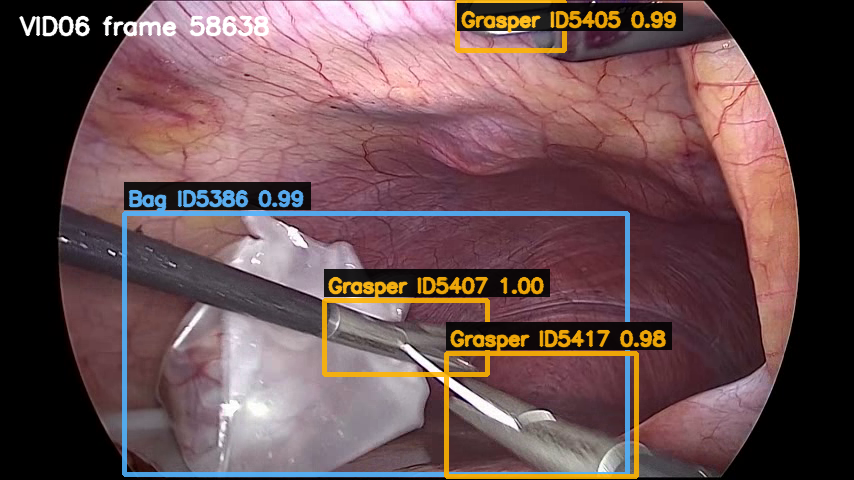
\includegraphics[width=0.75\textwidth]{assets/tracking_sample_1.png}\caption{Sample tracking output 1.}\end{figure}

\begin{figure}[H]\centering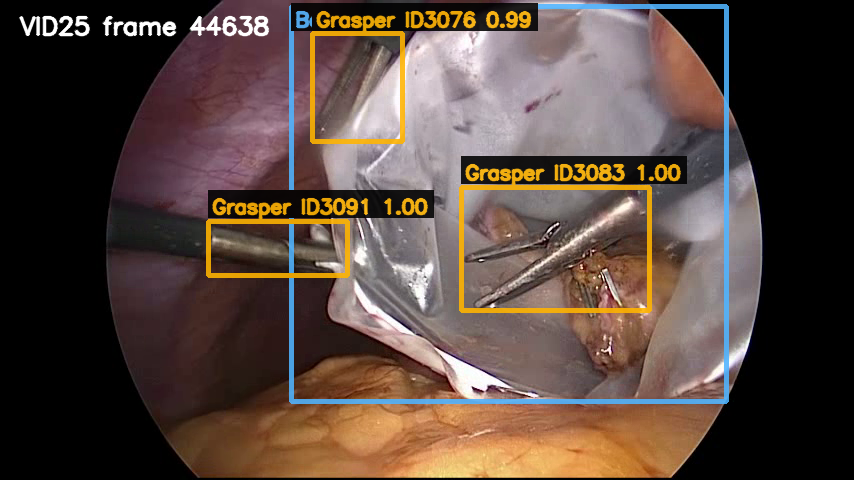
\includegraphics[width=0.75\textwidth]{assets/tracking_sample_2.png}\caption{Sample tracking output 2.}\end{figure}

\begin{figure}[H]\centering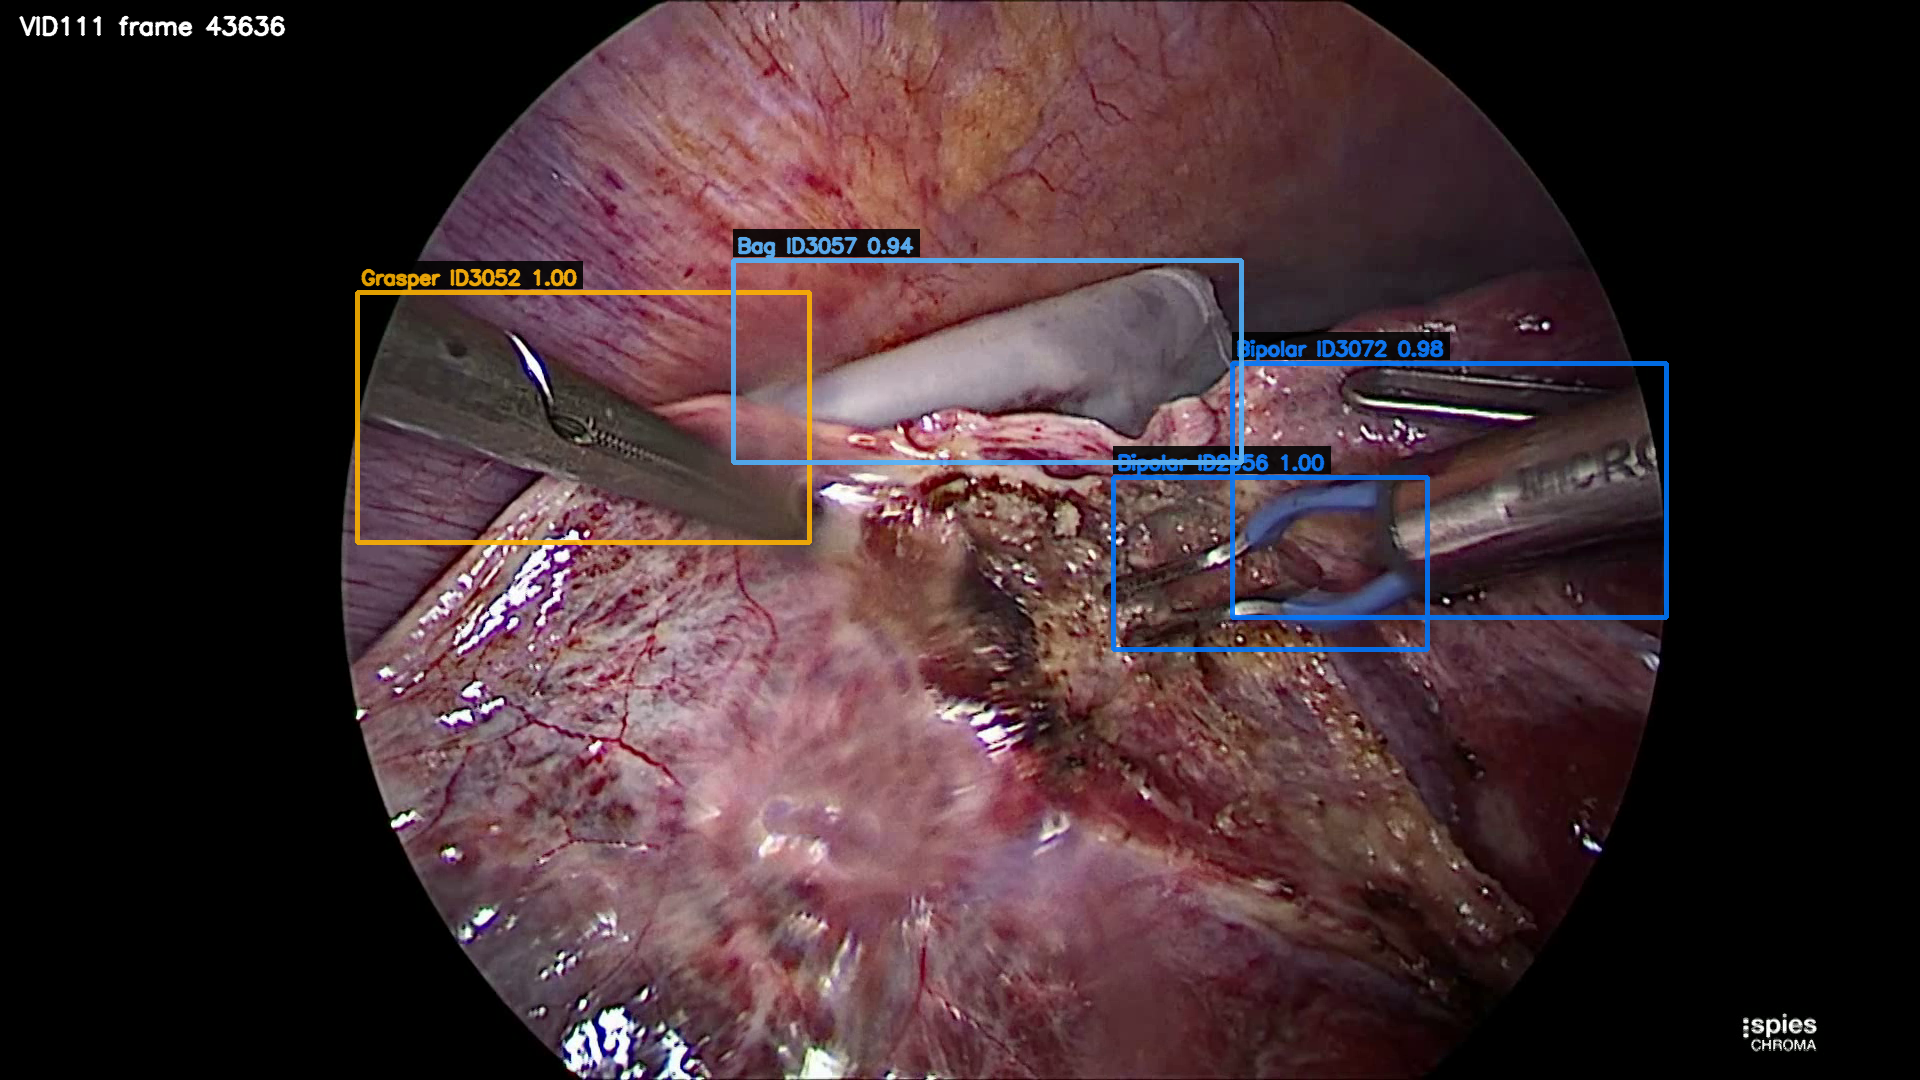
\includegraphics[width=0.75\textwidth]{assets/tracking_sample_3.png}\caption{Sample tracking output 3.}\end{figure}

\section{Conclusion}

This project documents the full path from YOLO11 baseline experiments to an EfficientDet-D0 and StrongSORT/EA-StrongSORT-oriented contribution for CholecTrack20. The final framework integrates transfer learning, EfficientNet-family detection, BiFPN feature-level attention, tracking-by-detection, StrongSORT identity association, and multi-perspective tracking evaluation. It also provides practical engineering contributions, including fast presets, streaming tracking, experiment logging, and paper-style metric outputs.

The main finding is that EfficientDet-D0 improved the internal detector baseline compared with YOLO11, but the improvement was not large enough to approach the strongest public CholecTrack20 detector results. The tracking benchmark confirmed the same conclusion at the sequence level. The pipeline works, produces valid MOT outputs, and can be evaluated across all three CholecTrack20 perspectives, but the final MOTA and IDF1 scores remain limited by detector quality and identity fragmentation.

The most important limitation is that the project did not yet implement the exact EfficientNetV2/ECA ReID replacement and GIoU association strategy described in the EA-StrongSORT reference paper. Instead, the current tracking stage uses a stable StrongSORT/OSNet implementation while the detector family was changed and evaluated. This was a reasonable staged design because detector quality was the clearest bottleneck. Still, a complete future version should implement the EA-StrongSORT ReID branch, compare OSNet versus EfficientNetV2/ECA embeddings, and measure whether GIoU association improves CholecTrack20 identity preservation.

Future work should proceed in three directions. First, detector training should be strengthened through class-aware sampling, rare-class augmentation, stronger CholecTrack20-specific training schedules, and possibly larger detector backbones if hardware permits. Second, the exact EA-StrongSORT modules should be implemented and tested after the detector becomes more reliable. Third, evaluation should include more detailed per-class and per-challenge tracking analysis so that improvements can be linked to specific surgical conditions. This staged plan turns the current result into a useful research baseline rather than a dead end.

\section*{References}

\begin{enumerate}

\item Aharon, N., Orfaig, R., \& Bobrovsky, B. Z. (2022). BoT-SORT: Robust associations multi-pedestrian tracking. arXiv preprint arXiv:2206.14651.

\item Bewley, A., Ge, Z., Ott, L., Ramos, F., \& Upcroft, B. (2016). Simple online and realtime tracking. Proceedings of the IEEE International Conference on Image Processing, 3464-3468.

\item Bochkovskiy, A., Wang, C. Y., \& Liao, H. Y. M. (2020). YOLOv4: Optimal speed and accuracy of object detection. arXiv preprint arXiv:2004.10934.

\item Du, Y., Song, Y., Yang, B., \& Zhao, Y. (2023). StrongSORT: Make DeepSORT great again. IEEE Transactions on Multimedia, 25, 8725-8737.

\item Ge, Z., Liu, S., Wang, F., Li, Z., \& Sun, J. (2021). YOLOX: Exceeding YOLO series in 2021. arXiv preprint arXiv:2107.08430.

\item Ghatwary, N., Amer, A., Fayed, S., Magdy, S., Hussein, A., Kadry, R., \& Abdelmaksoud, A. I. (n.d.). EA-StrongSORT: An efficient attention StrongSORT framework for detection-based tumor tracking in Cine-MRI TrackRAD2025 dataset.

\item Lin, T. Y., Goyal, P., Girshick, R., He, K., \& Dollar, P. (2017). Focal loss for dense object detection. Proceedings of the IEEE International Conference on Computer Vision, 2980-2988.

\item Luiten, J., Osep, A., Dendorfer, P., Torr, P. H. S., Geiger, A., Leal-Taixe, L., \& Leibe, B. (2021). HOTA: A higher order metric for evaluating multi-object tracking. International Journal of Computer Vision, 129, 548-578.

\item Nwoye, C. I., Elgohary, K., Srinivas, A., Zaid, F., Lavanchy, J. L., \& Padoy, N. (2025). CholecTrack20: A multi-perspective tracking dataset for surgical tools. Proceedings of the IEEE/CVF Conference on Computer Vision and Pattern Recognition.

\item Redmon, J., Divvala, S., Girshick, R., \& Farhadi, A. (2016). You only look once: Unified, real-time object detection. Proceedings of the IEEE Conference on Computer Vision and Pattern Recognition, 779-788.

\item Rezatofighi, H., Tsoi, N., Gwak, J., Sadeghian, A., Reid, I., \& Savarese, S. (2019). Generalized intersection over union: A metric and a loss for bounding box regression. Proceedings of the IEEE/CVF Conference on Computer Vision and Pattern Recognition, 658-666.

\item Tan, M., \& Le, Q. V. (2019). EfficientNet: Rethinking model scaling for convolutional neural networks. Proceedings of the International Conference on Machine Learning, 6105-6114.

\item Tan, M., Pang, R., \& Le, Q. V. (2020). EfficientDet: Scalable and efficient object detection. Proceedings of the IEEE/CVF Conference on Computer Vision and Pattern Recognition, 10781-10790.

\item Wang, Q., Wu, B., Zhu, P., Li, P., Zuo, W., \& Hu, Q. (2020). ECA-Net: Efficient channel attention for deep convolutional neural networks. Proceedings of the IEEE/CVF Conference on Computer Vision and Pattern Recognition, 11534-11542.

\item Wang, C. Y., Bochkovskiy, A., \& Liao, H. Y. M. (2023). YOLOv7: Trainable bag-of-freebies sets new state-of-the-art for real-time object detectors. Proceedings of the IEEE/CVF Conference on Computer Vision and Pattern Recognition, 7464-7475.

\item Wojke, N., Bewley, A., \& Paulus, D. (2017). Simple online and realtime tracking with a deep association metric. Proceedings of the IEEE International Conference on Image Processing, 3645-3649.

\item Zhang, Y., Sun, P., Jiang, Y., Yu, D., Weng, F., Yuan, Z., Luo, P., Liu, W., \& Wang, X. (2022). ByteTrack: Multi-object tracking by associating every detection box. Proceedings of the European Conference on Computer Vision, 1-21.

\end{enumerate}\end{document}